
\section{Estimates for number of Monte-Carlo samples needed}
\label{sec:experiments}

\begin{table}[!ht]
\centering
\begin{small}
\begin{tabular}{|p{2in}|l|l|p{0.75in}|p{0.75in}|p{0.75in}|}
\hline
 \textbf{Dataset} & \textbf{Nodes} & \textbf{Edges} & \textbf{Average clustering coefficient}
& \textbf{Transitivity} & \textbf{Degree assortativity}  \\ 
\hline
 Montgomery county social network (constructed by the methods of~\cite{barrett:wsc09,eubank:nature04}) & 75457 & 648667 & 0.5345 &  0.5087 & 0.3273\\
 ca-AstroPh~\cite{snap} & 18772 & 198110 & 0.6306 & 0.318 & 0.2051\\
 Enron email network~\cite{snap} & 36692 & 183831 & 0.4970 & 0.0853 & -0.11\\   
 Brightkite~\cite{snap} & 58228 & 214078 & 0.1723 & 0.1105 & 0.0108\\ 
Musae-facebook~\cite{snap} & 22470 & 171002 & 0.3597 & 0.2323 & 0.085\\ 
\hline
\end{tabular}
\end{small}
\caption{Datasets used in the empirical analysis of Monte-Carlo sampling.}
\label{tab:datasets}
\end{table}

Lemma \ref{lemma:mcmc-numinf} in Section \ref{sse:poly} shows that an 
$(\epsilon, \delta)$-approximation to the expected total number of infections 
in a set $S$ up to time $t$ can be estimated in polynomial time by a simple
Monte-Carlo sampling approach. Here, we examine the empirical complexity
of Monte-Carlo sampling of other problems in Table \ref{tab:prob_def}.
As an example, let $p^*$ be the exact probability for an instance of the \tTotInfs{} problem.
We use the approach of Dagum et al. \cite{dagum:focs95}, which gives an
$(\epsilon, \delta)$-approximation to $p^*$ using 
$N_{\epsilon, \delta} = O(N_{opt})$ samples, where
$N_{\epsilon, \delta}$ is the number of samples used by \cite{dagum:focs95}, and
$N_{opt}$ is the optimum number of Monte-Carlo samples that can give such an approximation
to $p^*$.  Figure \ref{fig:dagum-mcmc-montgomery}
shows $N_{\epsilon, \delta}$ as a function
of $t$ for the five different networks in Table~\ref{tab:datasets}, 
and different probability values, for 
$\epsilon = \delta=0.1$.
Since there is a huge variance in the infected fraction, instead of
choosing the transmission probability solely based on constraints on its expectation,
we consider the probability that the infected fraction is above a threshold.
Specifically, we consider a threshold of 15\%, and consider the value of $p$, so that
the probability that the fraction infected exceeds this threshold is close to 0.1
(referred to as ``low''), 0.4 (referred to as ``medium''), and 0.7 (referred to as ``high'').
For each network, and each probability value, we examine how $N_{\epsilon, \delta}$
varies with $t$, for a fixed value of $q$; three different values of $q$ are considered.
We note that $N_{\epsilon, \delta}$ reduce with $t$, and increase with $q$;
in general, they are quite high, which is an indication that the variance is pretty high.
Some of our main observations are
\begin{itemize}
\item
The number of samples $N_{\epsilon, \delta}$ generally drops very rapidly, as $t$
increases. It also increases with $q$. However, $N_{\epsilon, \delta}$ is not monotone,
in general, since the algorithm of \cite{dagum:focs95} is an estimator, and not an exact bound.
\item
In most of the networks, the number of samples needed for the low probability
setting is significantly higher than for medium or high probabilities. This is not
surprising, as the low probability leads to high variance.
\item
The Montgomery county social network needs the largest number of samples,
which suggests a significantly higher variance in the outbreak characteristics
in such networks, compared to other online social networks.
\end{itemize}

The large number of samples needed in many cases is further indication of the
empirical hardness of the forecasting problems studied in this paper.

\begin{figure}
\centering
%%\includegraphics[width=0.4\textwidth]{{dagum-0.0002}.pdf}
%%\includegraphics[width=0.4\textwidth]{{dagum-0.0004}.pdf}
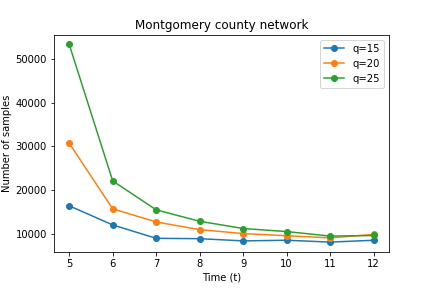
\includegraphics[width=0.3\textwidth]{{figs/montgomery_p0.0435}.png}
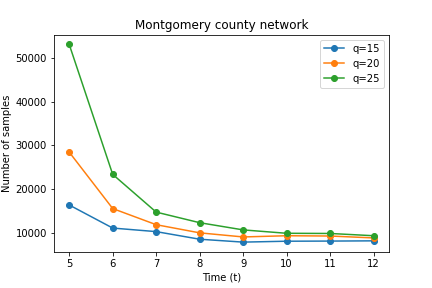
\includegraphics[width=0.3\textwidth]{{figs/montgomery_p0.044}.png}
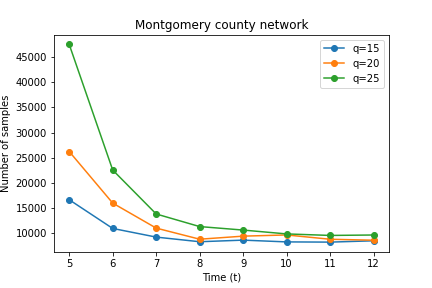
\includegraphics[width=0.3\textwidth]{{figs/montgomery_p0.0445}.png}
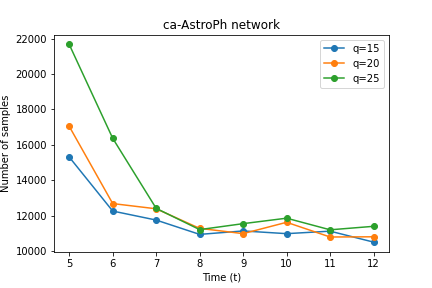
\includegraphics[width=0.3\textwidth]{{figs/ca-AstroPh_p0.0254}.png}
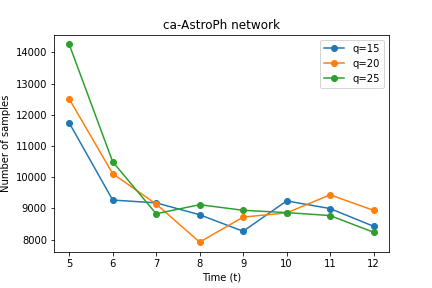
\includegraphics[width=0.3\textwidth]{{figs/ca-AstroPh_p0.03}.png}
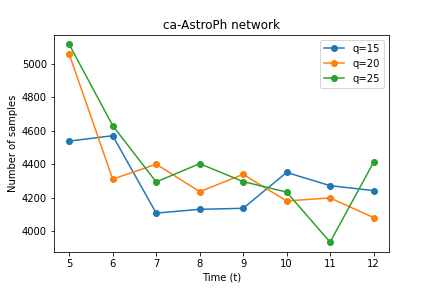
\includegraphics[width=0.3\textwidth]{{figs/ca-AstroPh_p0.06}.png}
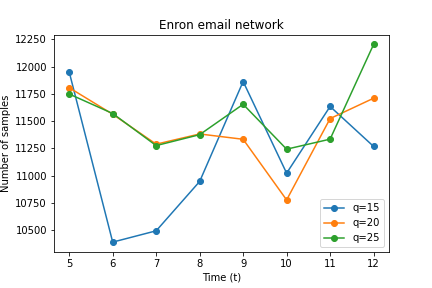
\includegraphics[width=0.3\textwidth]{{figs/email-Enron_p0.0498}.png}
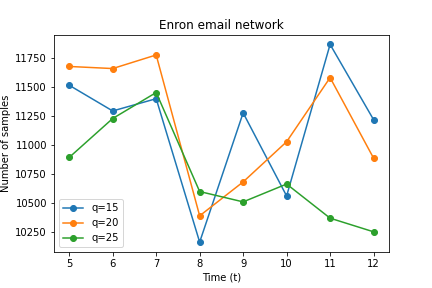
\includegraphics[width=0.3\textwidth]{{figs/email-Enron_p0.0515}.png}
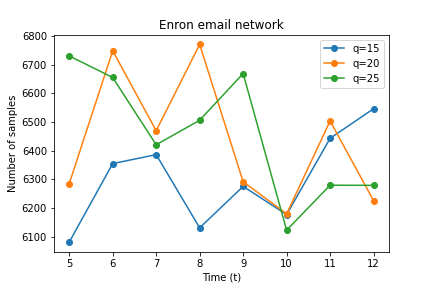
\includegraphics[width=0.3\textwidth]{{figs/email-Enron_p0.098}.png}
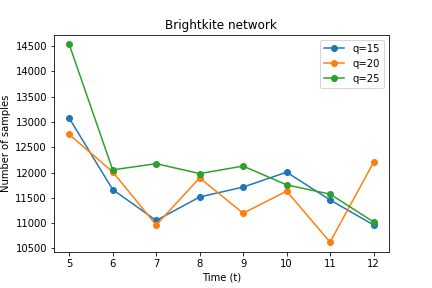
\includegraphics[width=0.3\textwidth]{{figs/loc-brightkite_p0.0693}.png}
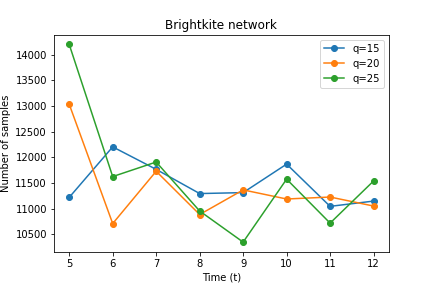
\includegraphics[width=0.3\textwidth]{{figs/loc-brightkite_p0.07045}.png}
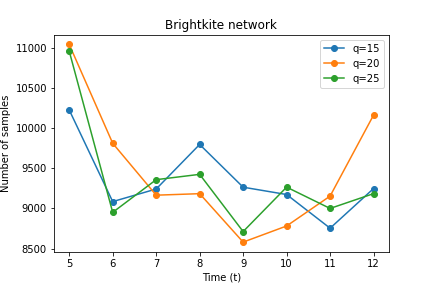
\includegraphics[width=0.3\textwidth]{{figs/loc-brightkite_p0.0852}.png}
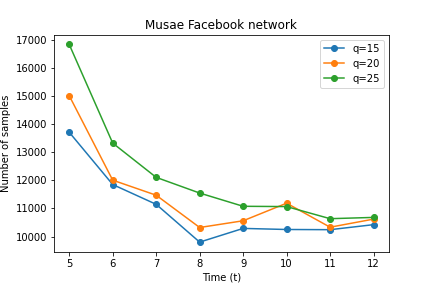
\includegraphics[width=0.3\textwidth]{{figs/musae_facebook_p0.0388}.png}
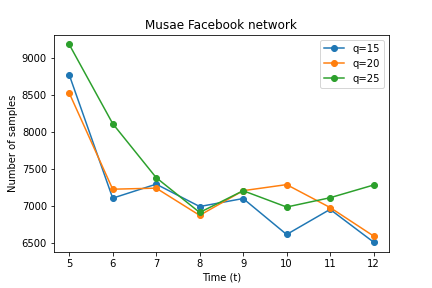
\includegraphics[width=0.3\textwidth]{{figs/musae_facebook_p0.055}.png}
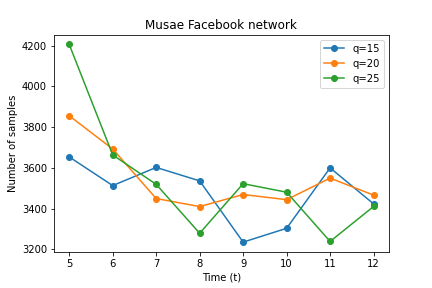
\includegraphics[width=0.3\textwidth]{{figs/musae_facebook_p0.118}.png}
\caption{Number of Monte-Carlo samples using the approach of Dagum et al. \cite{dagum:focs95}
on five different types of networks, as summarized in Table~\ref{tab:datasets}:
a social contact network for Montgomery county, VA, constructed using the approach of
\cite{eubank:nature04, barrett:wsc09} (Row 1),
ca-AstroPh (Row 2), Enron email network (Row 3),
Brightkite location network (Row 4), Facebook network (Row 5).
For each network, we choose three probability values, which ensure that the fraction
of infections is at least 15\% with varying
probability values: low$\sim 0.1$ (left), medium$\sim 0.4$ (middle), and high$\sim 0.7$ (right).
}
\label{fig:dagum-mcmc-montgomery}
\end{figure}

%%%%%%%%% 
\iffalse
\begin{figure}
\centering
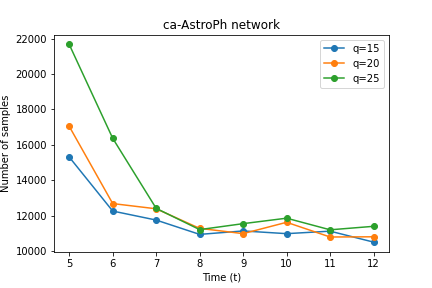
\includegraphics[width=0.3\textwidth]{{figs/ca-AstroPh_p0.0254}.png}
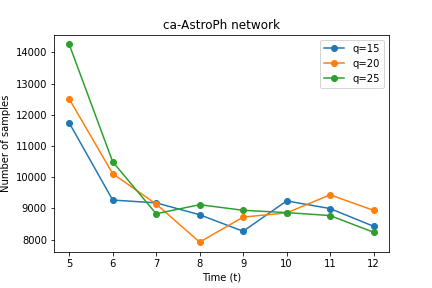
\includegraphics[width=0.3\textwidth]{{figs/ca-AstroPh_p0.03}.png}
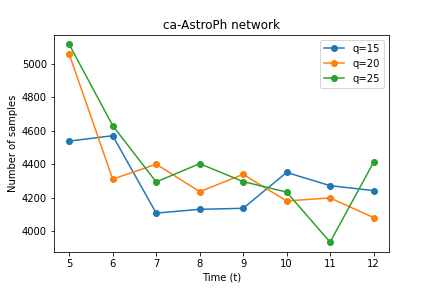
\includegraphics[width=0.3\textwidth]{{figs/ca-AstroPh_p0.06}.png}
\caption{Number of Monte-Carlo samples using the approach of Dagum et al. \cite{dagum:focs95}
for the ca-AstroPh network,
for a transmission probability, such that the expected number of infections 
is around 15\% of the total number of nodes with varying
probability values: low (left), medium (middle), and high (right).
}
\label{fig:dagum-mcmc-ca-astroph}
\end{figure}


\begin{figure}
\centering
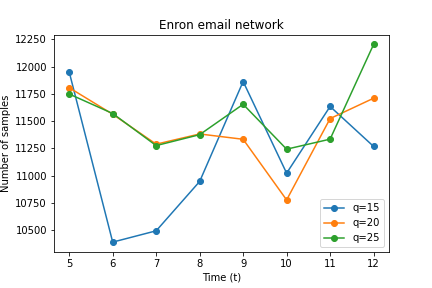
\includegraphics[width=0.3\textwidth]{{figs/email-Enron_p0.0498}.png}
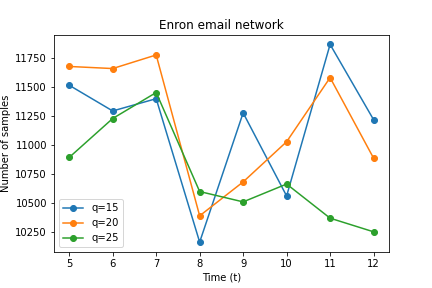
\includegraphics[width=0.3\textwidth]{{figs/email-Enron_p0.0515}.png}
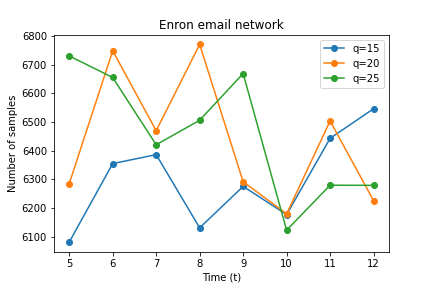
\includegraphics[width=0.3\textwidth]{{figs/email-Enron_p0.098}.png}
\caption{Number of Monte-Carlo samples using the approach of Dagum et al. \cite{dagum:focs95}
for the Enron email network,
for a transmission probability, such that the expected number of infections 
is around 15\% of the total number of nodes with varying
probability values: low (left), medium (middle), and high (right).
}
\label{fig:dagum-mcmc-enron}
\end{figure}


\begin{figure}
\centering
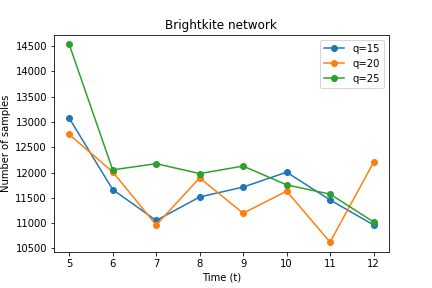
\includegraphics[width=0.3\textwidth]{{figs/loc-brightkite_p0.0693}.png}
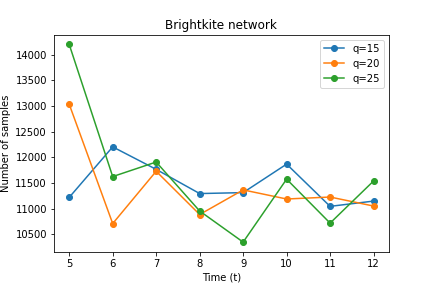
\includegraphics[width=0.3\textwidth]{{figs/loc-brightkite_p0.07045}.png}
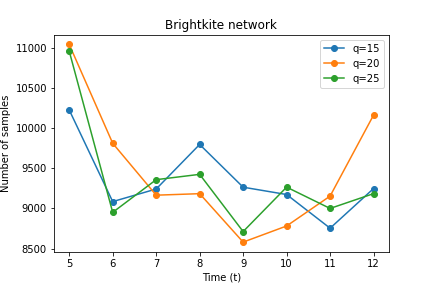
\includegraphics[width=0.3\textwidth]{{figs/loc-brightkite_p0.0852}.png}
\caption{Number of Monte-Carlo samples using the approach of Dagum et al. \cite{dagum:focs95}
for the Brightkite location network,
for a transmission probability, such that the expected number of infections 
is around 15\% of the total number of nodes with varying
probability values: low (left), medium (middle), and high (right).
}
\label{fig:dagum-mcmc-brightkite}
\end{figure}


\begin{figure}
\centering
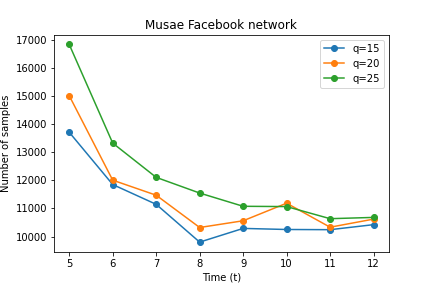
\includegraphics[width=0.3\textwidth]{{figs/musae_facebook_p0.0388}.png}
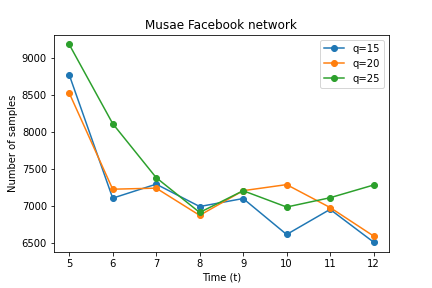
\includegraphics[width=0.3\textwidth]{{figs/musae_facebook_p0.055}.png}
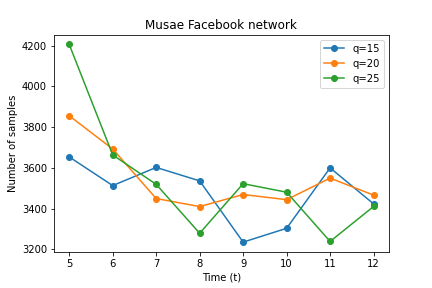
\includegraphics[width=0.3\textwidth]{{figs/musae_facebook_p0.118}.png}
\caption{Number of Monte-Carlo samples using the approach of Dagum et al. \cite{dagum:focs95}
for the Musae Facebook network,
for a transmission probability, such that the expected number of infections 
is around 15\% of the total number of nodes with varying
probability values: low (left), medium (middle), and high (right).
}
\label{fig:dagum-mcmc-facebook}
\end{figure}
\fi

